\chapter{Exploratory Testing Insights}
\markboth{Exploratory Testing Insights}{}

\section{Introduction}
This chapter presents the first two sprints carried out during the internship at SeekMake. The sprints were focused on exploratory testing of the web application.

\section{Background}

At the beginning of the first sprint, the team was introduced to the SeekMake web application.

The team was given a brief overview of the application and its functionalities. The team was also provided with access to the application and the necessary documentation.

\section{Testing Approach}
The QA team used exploratory testing to test the SeekMake web application. The QA team explored the application without any pre-defined test cases or scripts. The team used their knowledge and experience to test the application and identify any issues or bugs.

\subsection{Micro Frontends Architecture}

The SeekMake web application is built using the Micro Frontends architecture.

The idea behind Micro Frontends is to think about a website or web app as a composition of features which are owned by independent teams. Each team has a distinct area of business or mission it cares about and specialises in. A team is cross functional and develops its features end-to-end, from database to user interface. \cite{microfrontends}

\begin{figure}[H]
    \centering
    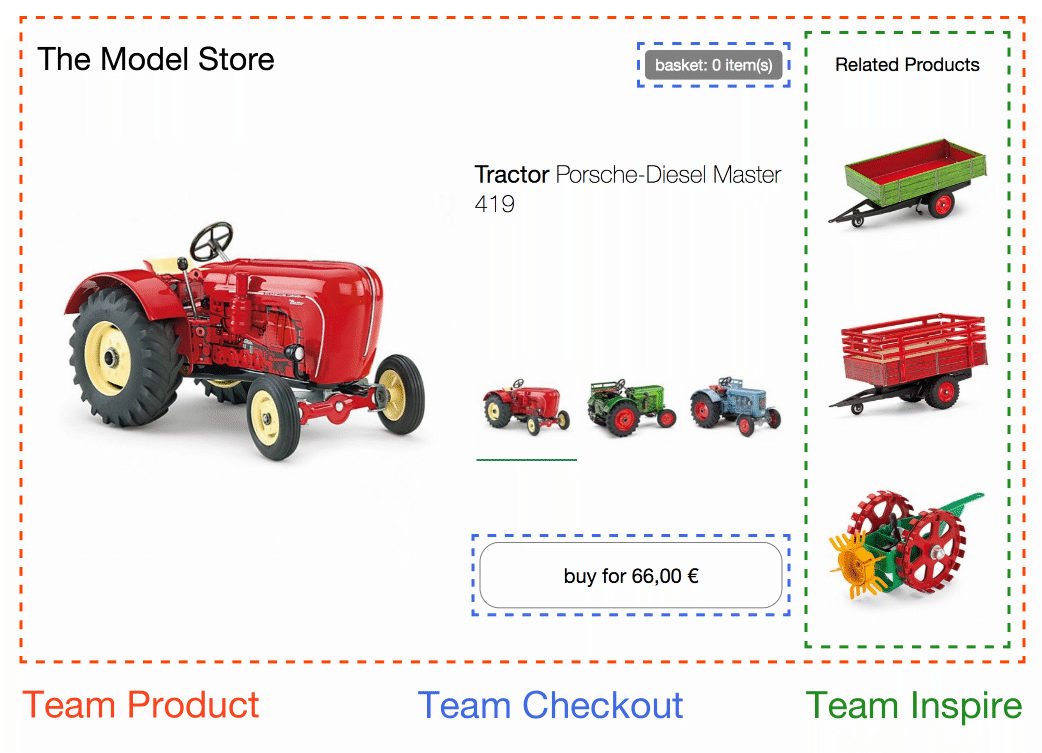
\includegraphics[width=0.8\textwidth]{project/images/three-teams.png}
    \caption{A figure demonstrating an example of Micro Frontends Architecture}
    \label{fig:microfrontends}
\end{figure}

This architecture allows the development team to work on different parts of the application independently, without affecting other parts of the application. It also allows the team to scale the application easily by adding new Micro Frontends.

The QA team was tasked with exploring the Micro Frontends of the application and identifying any issues or bugs. The team was also asked to provide feedback on the usability and user experience of the application.

\subsection{Checklists}
The QA team created checklists to guide the exploratory testing of the Micro Frontends, where each checklist focused on a specific Micro Frontend.

The checklists included a list of features and functionalities that needed to be tested, as well as a list of common issues and bugs that could be encountered.

\subsubsection{GitHub Issues}

The QA team used GitHub Issues to track bugs and issues identified during the exploratory testing.

The team created a new issue for each bug or issue identified, and assigned it to the relevant team member.

The team then worked together using collaboration tools like Microsoft Teams to resolve the issue and verify the fix.

\begin{figure}[H]
    \centering
    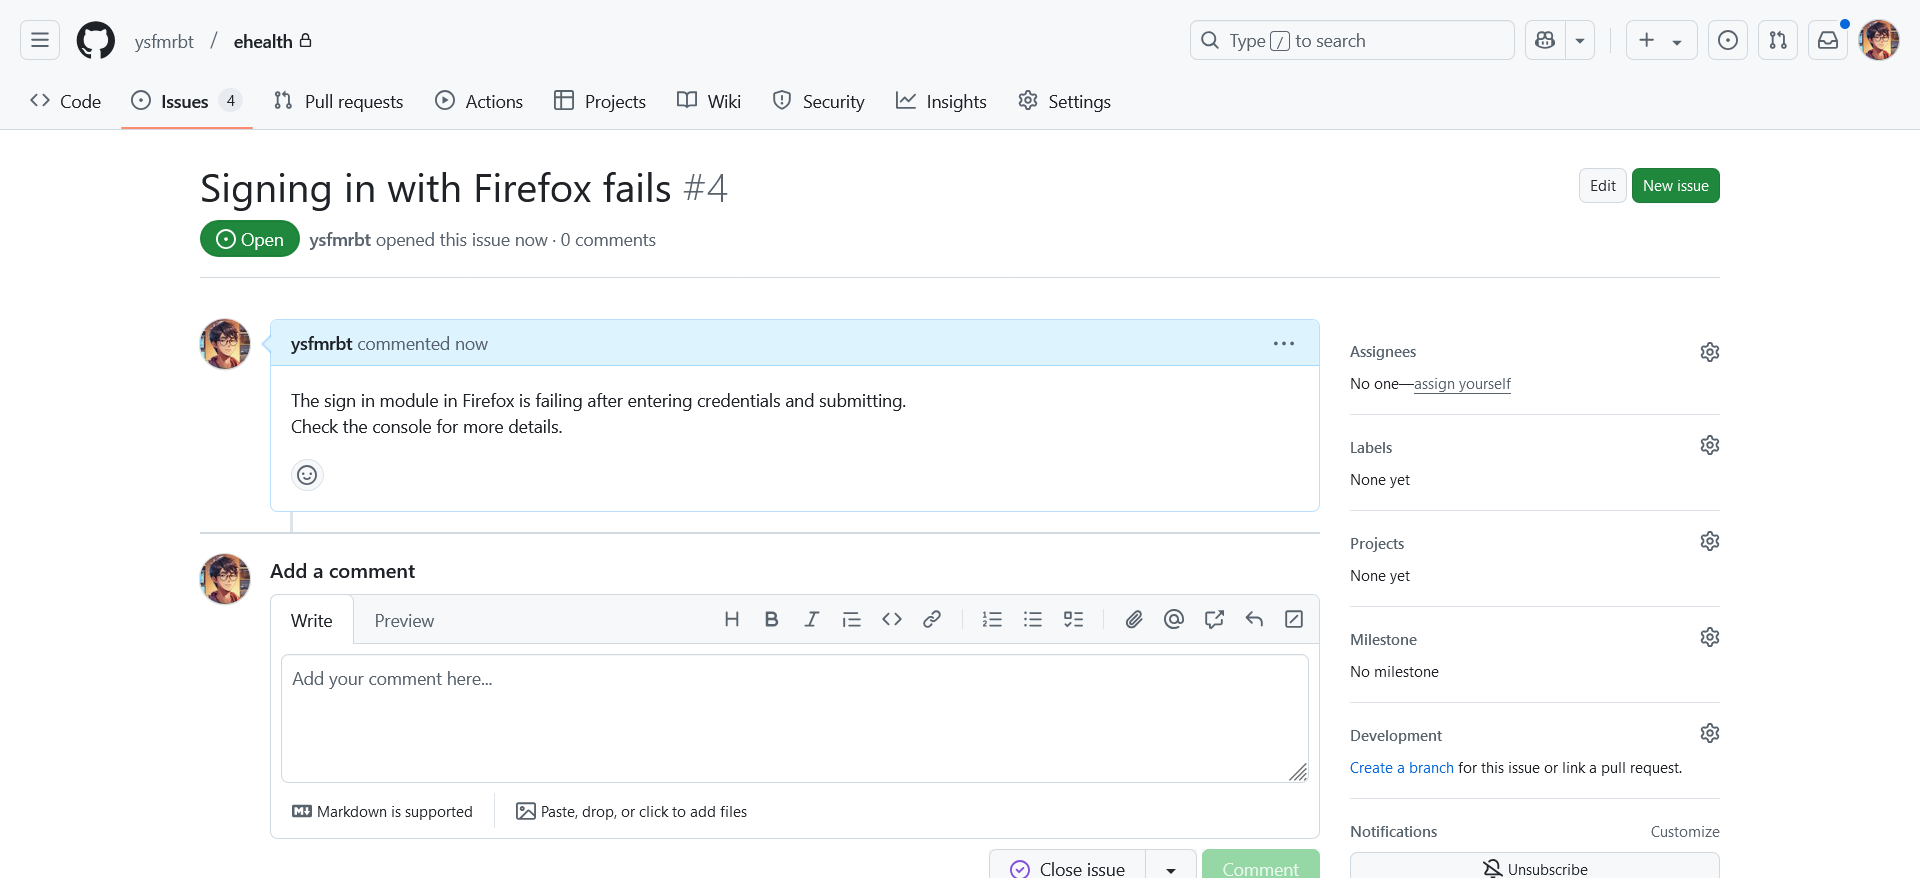
\includegraphics[width=\textwidth]{project/images/github-issue.png}
    \caption{An example of a GitHub Issue.}
    \label{fig:github-issue}
\end{figure}

The use of GitHub Issues allowed the team to track the progress of bug fixes and ensure that all issues were resolved before the end of the sprints.

\subsubsection{Confirmation Testing}

Confirmation testing confirms that an original defect has been successfully fixed. \cite{istqbctfl4.0.1}

Depending on the risk, one can test the fixed version of the software in several ways, including executing all tests that previously have failed due to the defect, or, also by adding new tests to cover any changes that were needed to fix the defect.  \cite{istqbctfl4.0.1}

The QA team performed confirmation testing to verify that all bugs and issues identified during the exploratory testing had been resolved.

\begin{figure}[H]
    \centering
    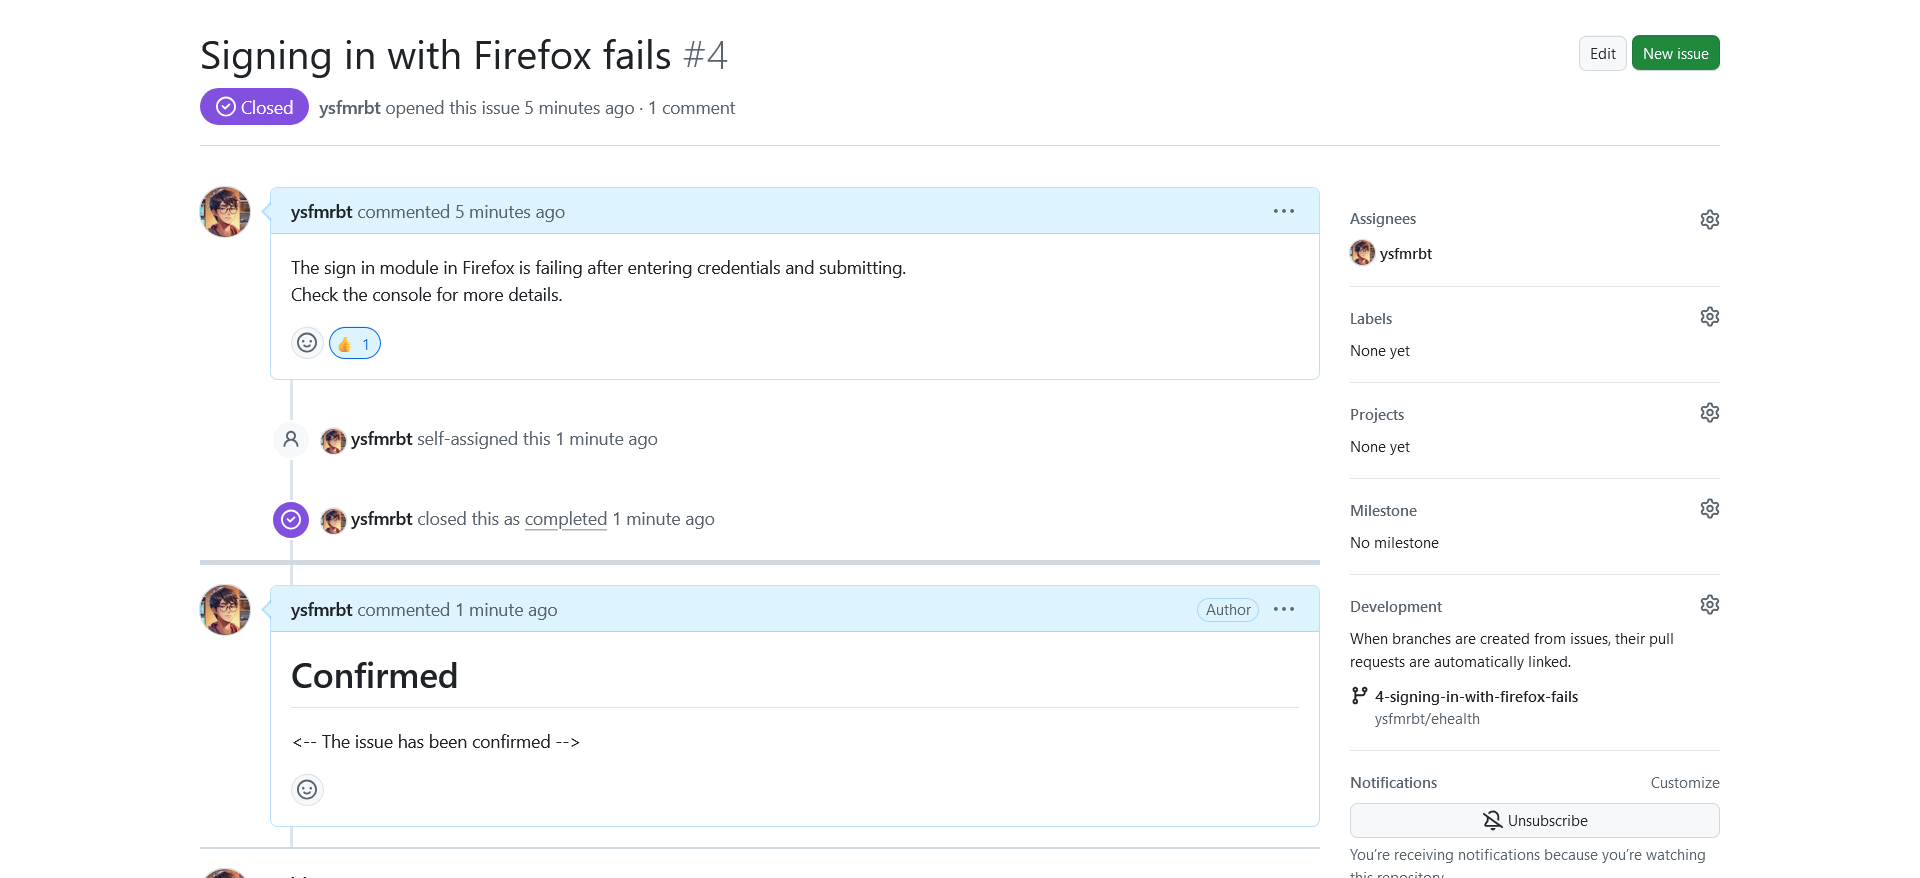
\includegraphics[width=\textwidth]{project/images/issue-confirmed.png}
    \caption{Issue confirmation.}
    \label{fig:issue-confirmed}
\end{figure}

To submit a confirmation test, the QA team followed these steps:

\begin{enumerate}
    \item Comment on the GitHub issue where the problem was reported.
    \item Attach a media (image or video) demonstrating the resolution of the problem.
    \item Close the issue to mark it as completed.
\end{enumerate}

\subsubsection{Manual Regression Testing}

Regression testing confirms that no adverse consequences have been caused by a change, including a fix that has already been confirmation tested. These adverse consequences could affect the same component where the change was made, other components in the same system, or even other connected systems. \cite{istqbctfl4.0.1}

The QA team performed manual regression testing to ensure that the bug fixes did not introduce any new issues or bugs.

\begin{figure}[H]
    \centering
    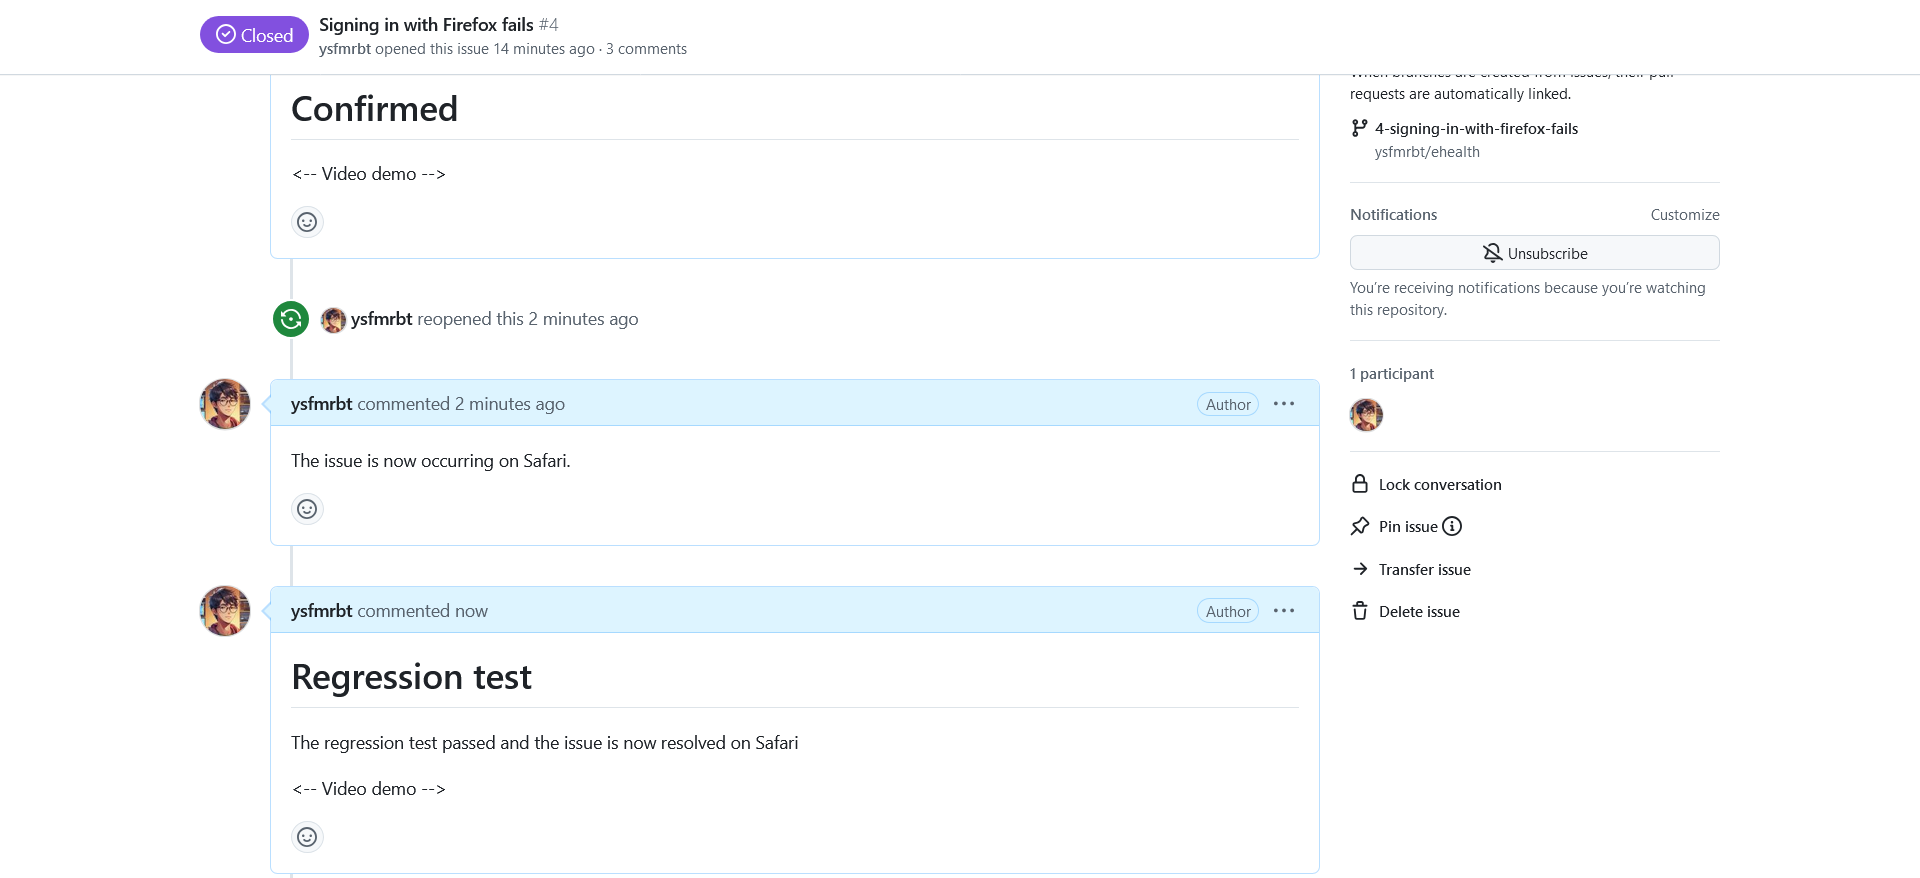
\includegraphics[width=\textwidth]{project/images/regression-test.png}
    \caption{Regression test.}
    \label{fig:regression-test}
\end{figure}

In the same way, to submit a manual regression test, the QA team followed these steps:

\begin{enumerate}
    \item Re-comment on and open the the GitHub issue where the problem was originally confirmed as resolved.
    \item Attach a media (image or video) demonstrating the resolution of the problem.
    \item Close the issue to mark it as completed.
\end{enumerate}
\section{Web Application Environment}

The SeekMake web application was deployed in different environments, including:

\subsection{Production}

The production environment is the live environment where the application is accessed by users. The production environment is deployed for using the application in a real-world scenario, and is monitored for performance and stability.

At the end of the sprints, the QA team deployed the application to the production environment for user acceptance testing.

The QA team used the production environment to test the application in a real-world scenario, and to identify any issues or bugs that were not present in the staging environment.

\subsection{Staging}

The staging environment is used for testing the application before it is deployed to production. The staging environment is an exact replica of the production environment, with the same configuration and data.

The QA team used the staging environment to test the application and identify any issues or bugs before it was deployed to production.

\subsection{Development}

The development environment is used by the development team to work on new features and bug fixes. The development environment is separate from the staging and production environments, and is used for testing changes before they are merged into the staging environment.

The QA team used the development environment to test new features and bug fixes before they were deployed to staging.

\section{Testing Results}

The QA team identified several bugs and issues during the exploratory testing of the SeekMake web application.

The bugs and issues were prioritised based on their severity and impact on the application and users. The team worked together to resolve the bugs and issues before the end of the sprints.

\subsection{Bugs and Issues}

The bugs and issues identified during the exploratory testing included:

\begin{itemize}
    \item Broken links (e.g. links that do not work or lead to the wrong page)
          Two examples of broken links are:
          \begin{itemize}
              \item The "Contact Us" link on the homepage redirected to the "About Us" page.
              \item The "Terms and Conditions" link on the checkout page redirected to a 404 error page.
          \end{itemize}
    \item Incorrect data (e.g. data that is missing or incorrect)
          \begin{figure}[H]
              \centering
              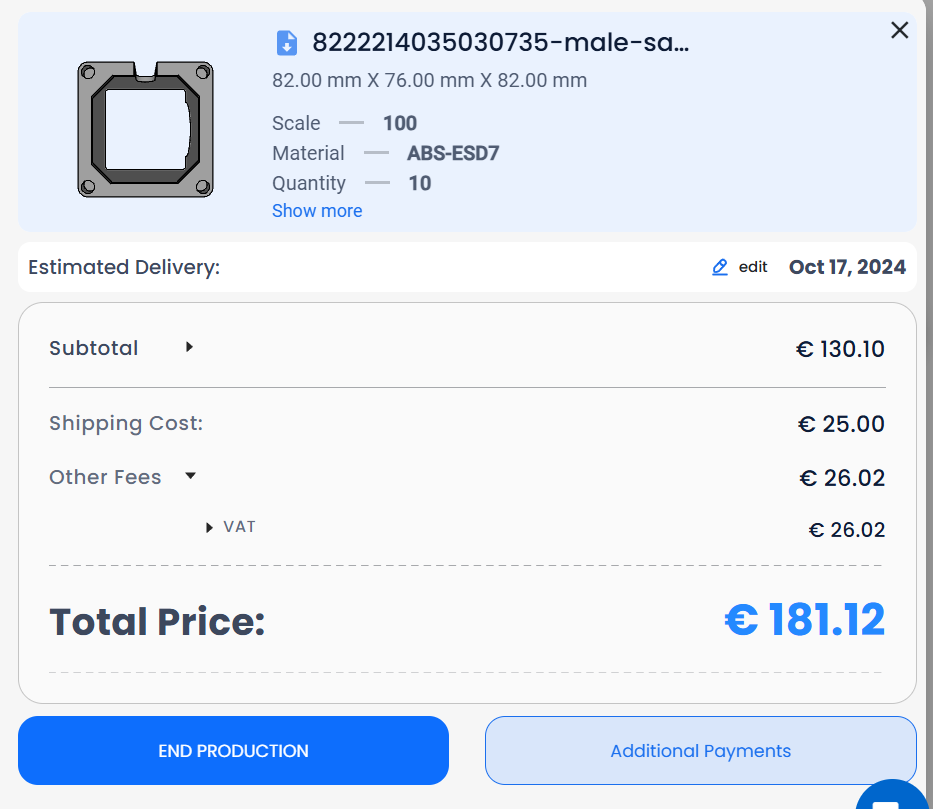
\includegraphics[width=0.5\textwidth]{project/images/incorrect-data.png}
              \caption{An example of incorrect data (Total price should be 181.02 instead of 181.12).}
              \label{fig:incorrect-data}
          \end{figure}
    \item Missing features (e.g. features that are not implemented or are not working as expected). An example of a missing feature that was encountered in SeekMake, is that users from certain countries were not able to complete the payment process.
    \item Performance issues (e.g. slow loading times or unresponsive pages). At the start of the sprint, the application took 10 seconds on average to load the homepage. After the sprint, the application took 5 seconds on average to load the homepage.
    \item Usability issues (e.g. poor navigation, confusing layout)
          \begin{figure}[H]
              \centering
              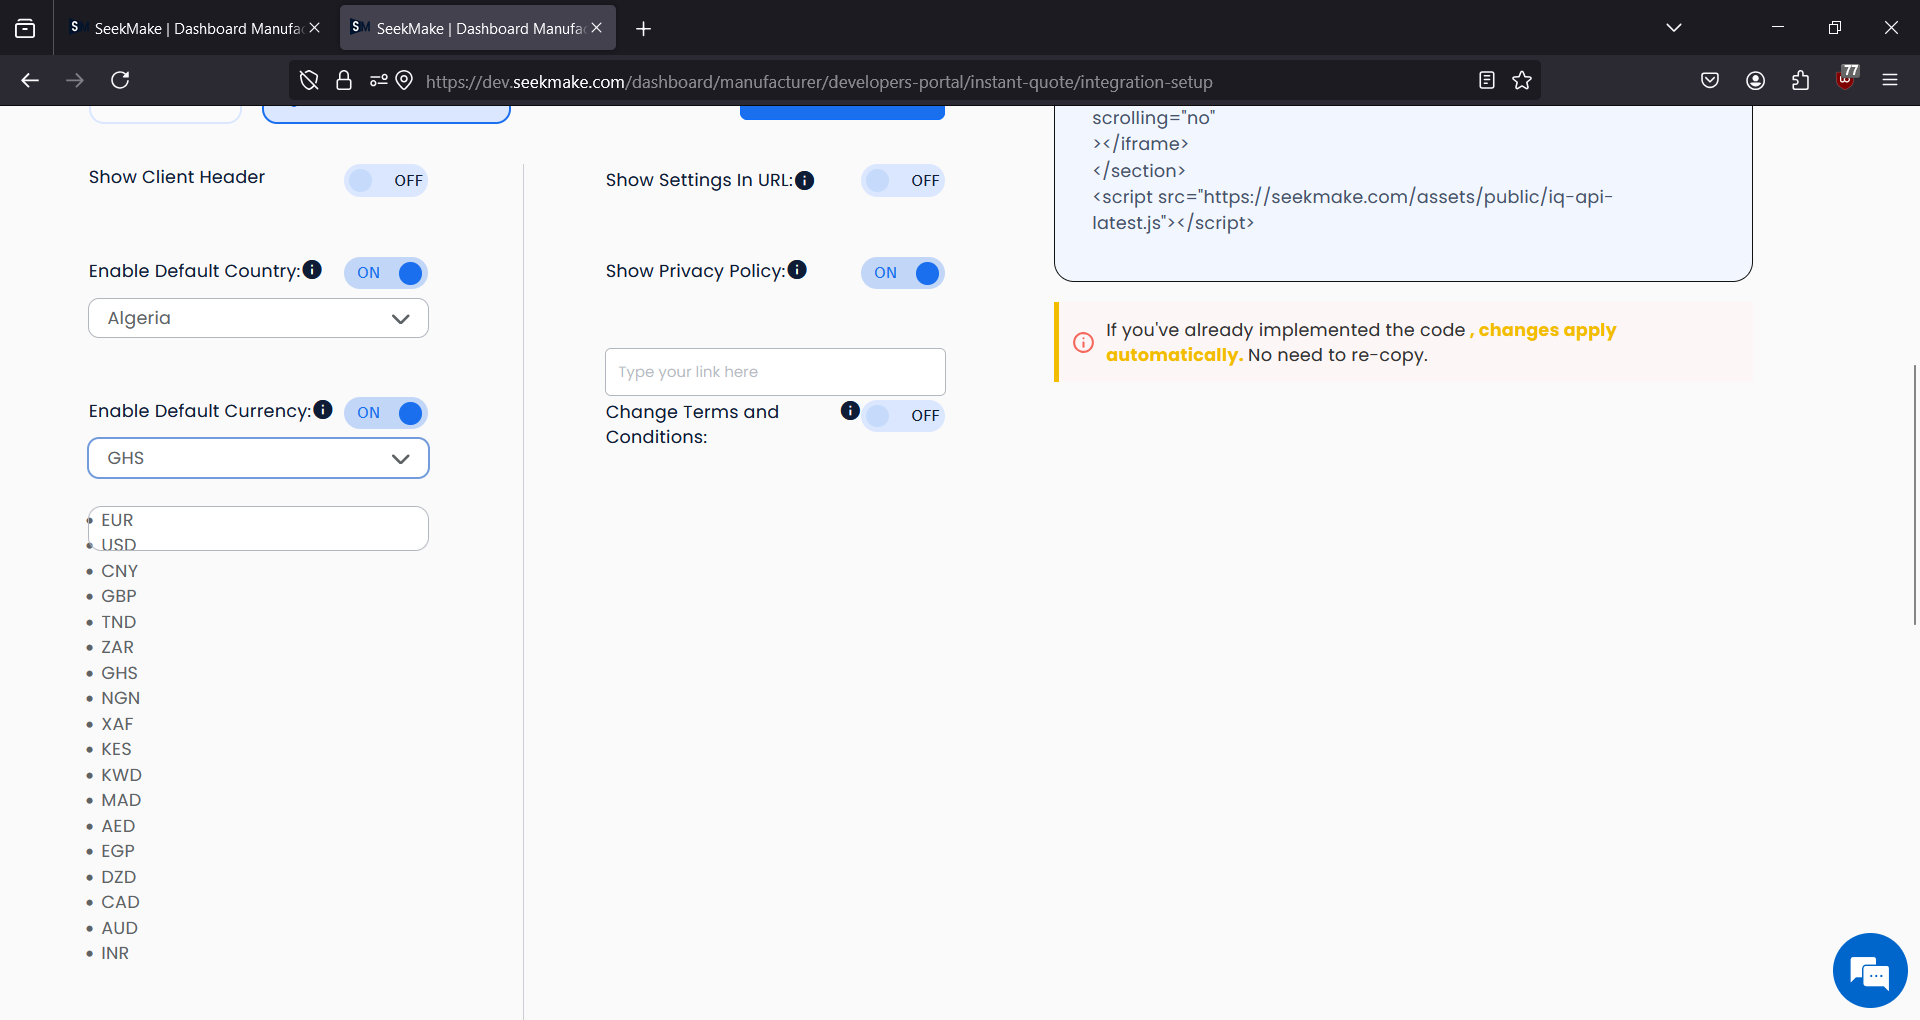
\includegraphics[width=\textwidth]{project/images/dropdown-broken.png}
              \caption{An example of a dropdown not fully implemented.}
              \label{fig:dropdown-broken}
          \end{figure}
    \item Security vulnerabilities (e.g. unprotected data). At the start of the sprint, a user could access the manufacturer dashboard by changing the URL. After the sprint, the manufacturer dashboard required the user to switch to a manufacturer account.
    \item Compatibility issues (e.g. the application does not work on certain devices or browsers). At the start of the sprint, the application did not work properly on Safari browser. After the sprint, the application worked on Safari.
\end{itemize}

The following are examples of how the bugs and issues were prioritised:
\begin{itemize}
    \item Critical: Payment gateway failed to process certain transactions.
    \item Major: Navigation links redirected to incorrect pages.
    \item Minor: Text alignment issues on smaller screen resolutions.
\end{itemize}
\section{Summary}

The first two sprints focused on exploratory testing of the SeekMake web application. The QA team used exploratory testing to test the Micro Frontends of the application and identify bugs and issues.

The team created checklists to guide the exploratory testing, and used GitHub Issues to track bugs and issues. The team performed confirmation testing and manual regression testing to verify that all bugs and issues were resolved.

The QA team identified several bugs and issues during the exploratory testing, and worked together to resolve them before the end of the sprints.

In the next sprint, the team will focus on end-to-end testing of the SeekMake web application.